\subsection*{Simple Model}

        The simplest possible model is the one in which the number of nucleotides determines the read duration,
        possibly with some constant term for getting started.  To consider this, we start with a scatterplot of
        bases against time with a linear fit.

        \begin{centering}
        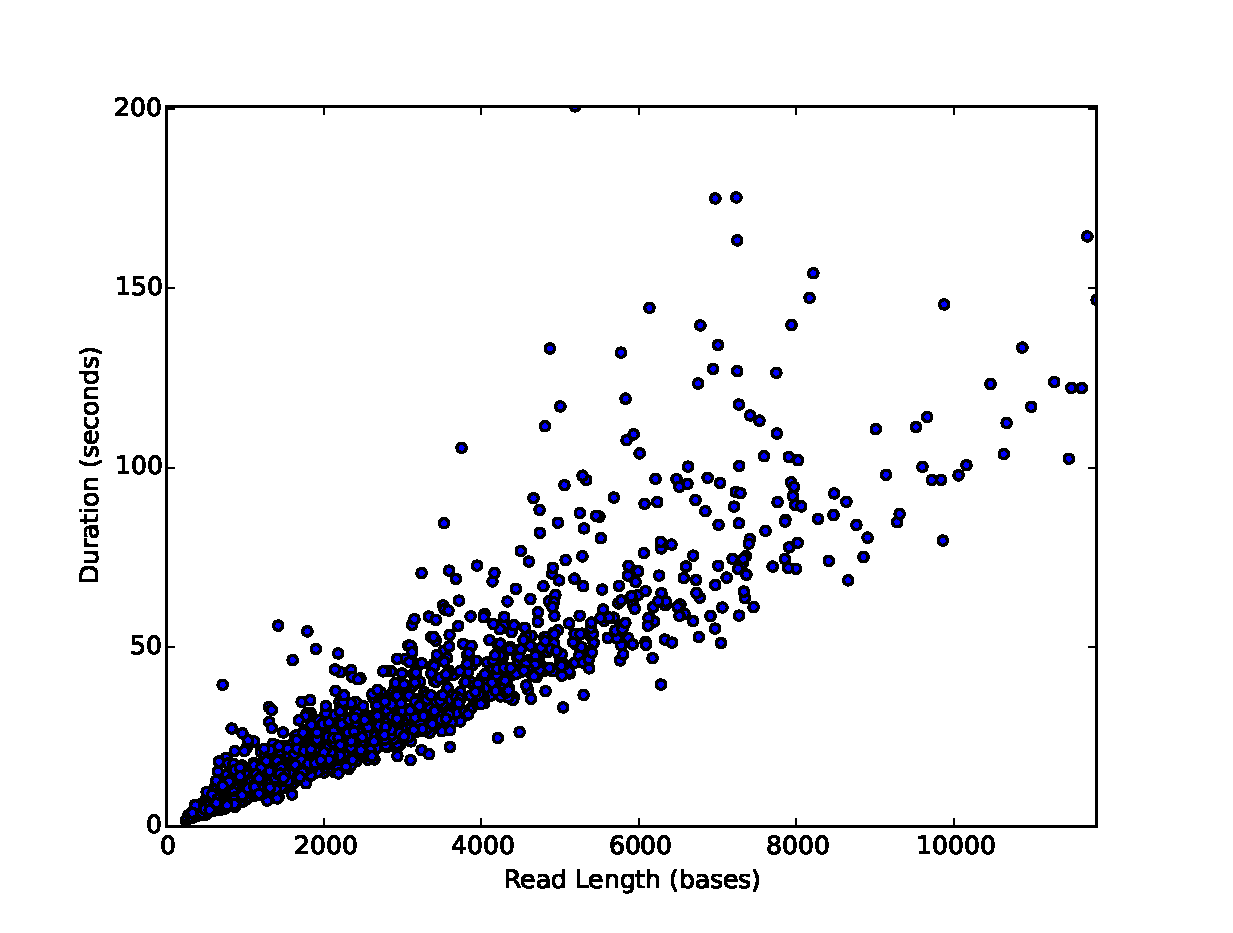
\includegraphics[width=\textwidth]{part11scatterbd}
        \end{centering}

        We might be tempted to include a constant term in our fitting, but as should be apparent, it would be
        negative.  How long it would take to sequence an extremely short read is unclear.  Fortunately, there 
        are none in our sample.

        \newpage
        This allows us to construct a trivial (and still pretty effective) model based on a fixed cost per nucleotide.

        Cost per nucleotide: 11.25ms
        
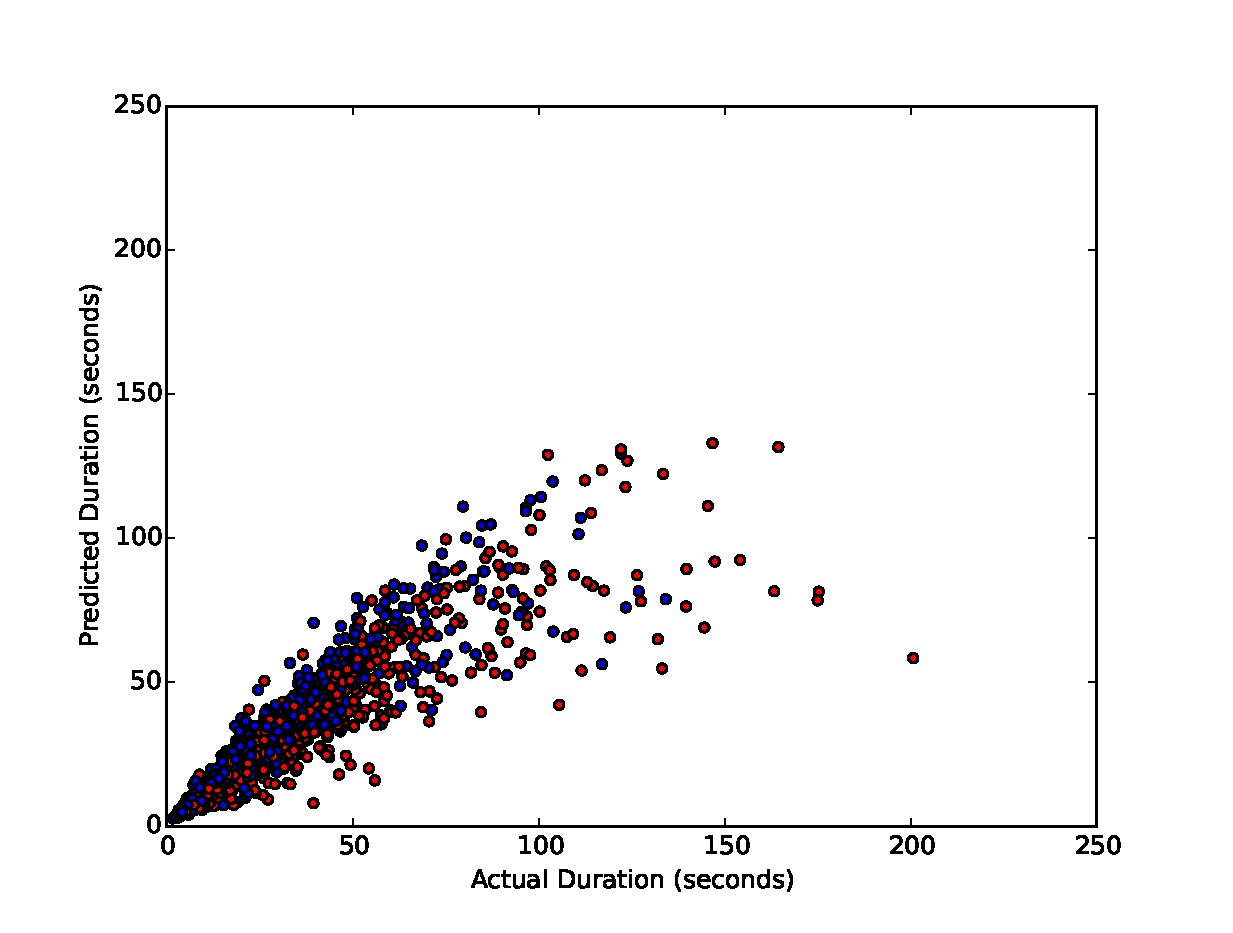
\includegraphics[width=\textwidth]{part11scatter0mer}

$r^2=0.84$


(Red circles are template strand; blue are complement.  There appears to be no significant difference between them.)

\newpage
\subsection*{Nucleotide Model}
A slightly more complex model uses a differend cost for each type of nucleotide: 
A=32ms 
C=-07ms 
G=04ms 
T=12ms 


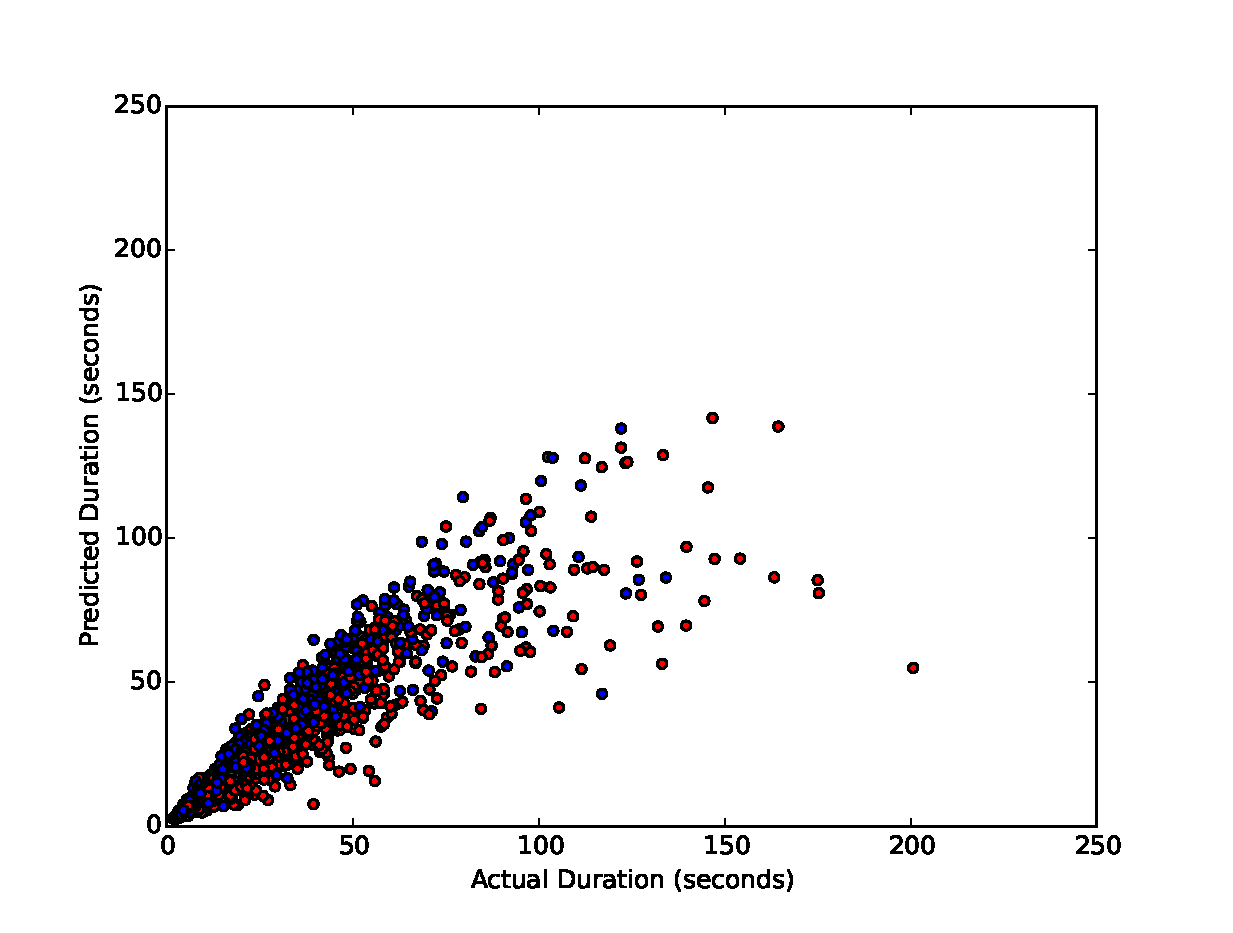
\includegraphics[width=\textwidth]{part11scatter1mer}

$r^2=0.84$


        \newpage
        \subsection*{2mer Model}
        \begin{wrapfigure}{R}{2in}
        \vspace{-50pt}
        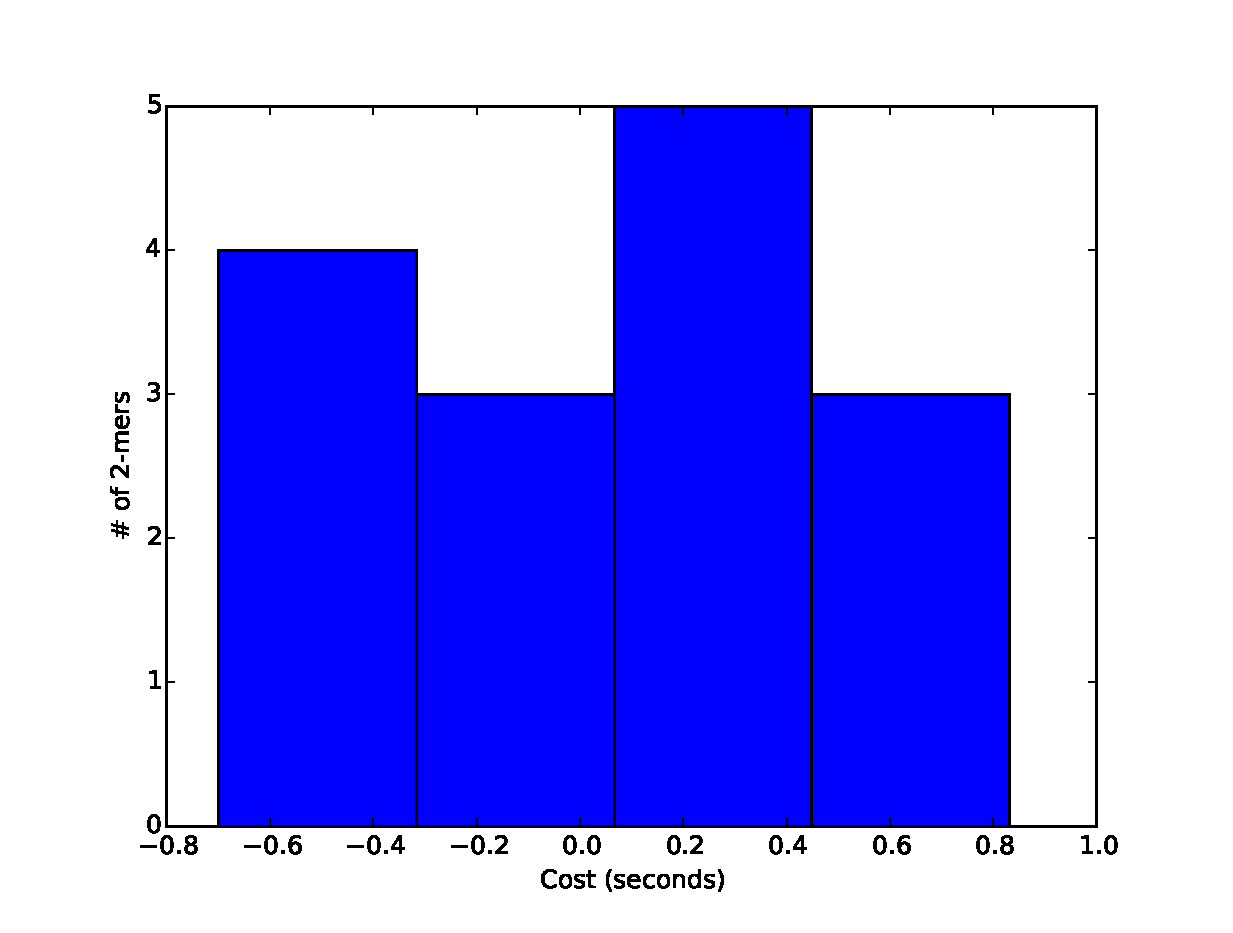
\includegraphics[width=3in]{part11hist2}
        \vspace{-70pt}
        \end{wrapfigure}
        We can use a model in which each the time to extend by one nucleotide is determined by the 2-mer in the middle of the
        pore.  We can not list all the costs, but here's a histogram:

        \vspace{1.5in}

        And here's the resulting predictions:
        
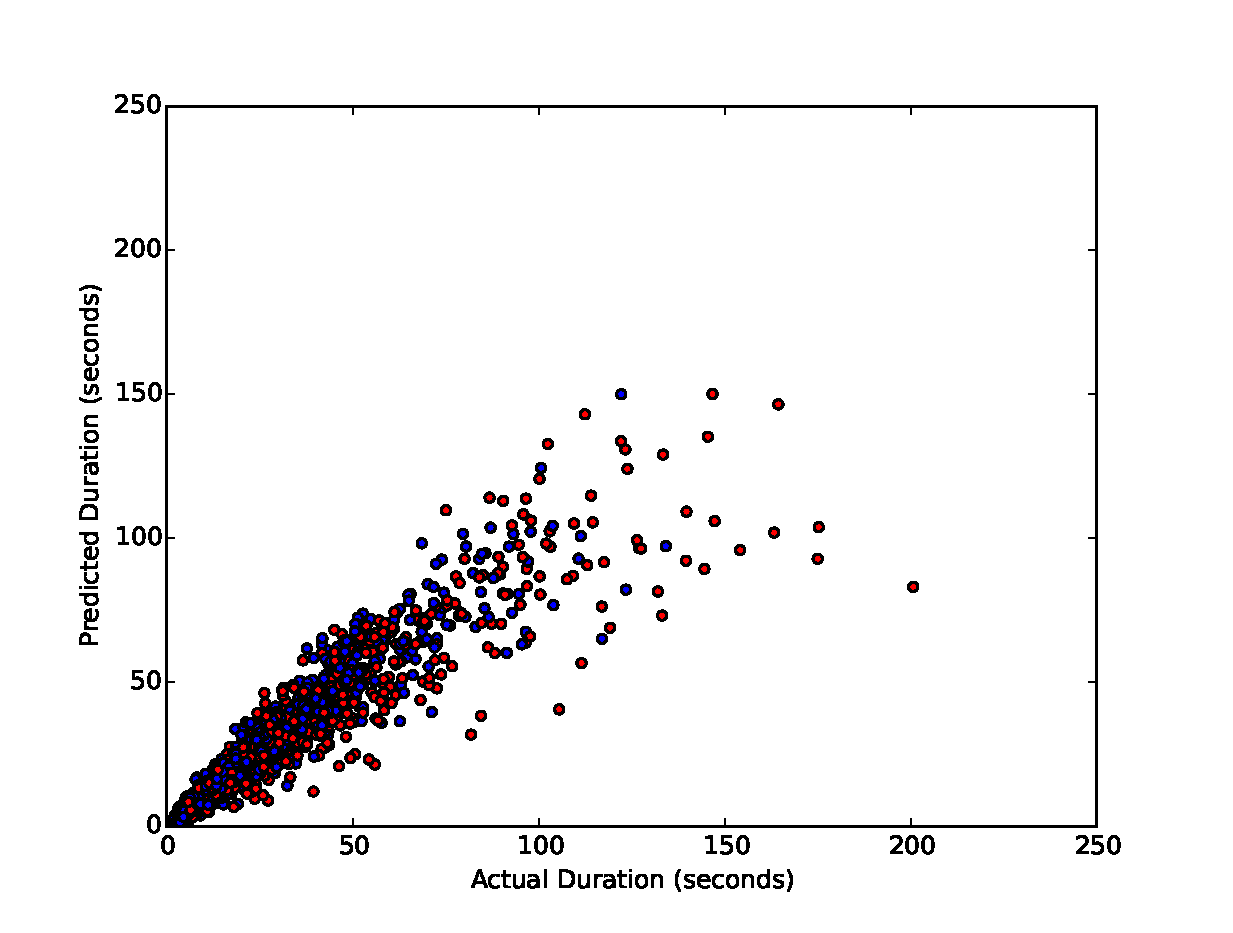
\includegraphics[width=\textwidth]{part11scatter2mer}

$r^2=0.88$


        \newpage
        \subsection*{3mer Model}
        \begin{wrapfigure}{R}{2in}
        \vspace{-50pt}
        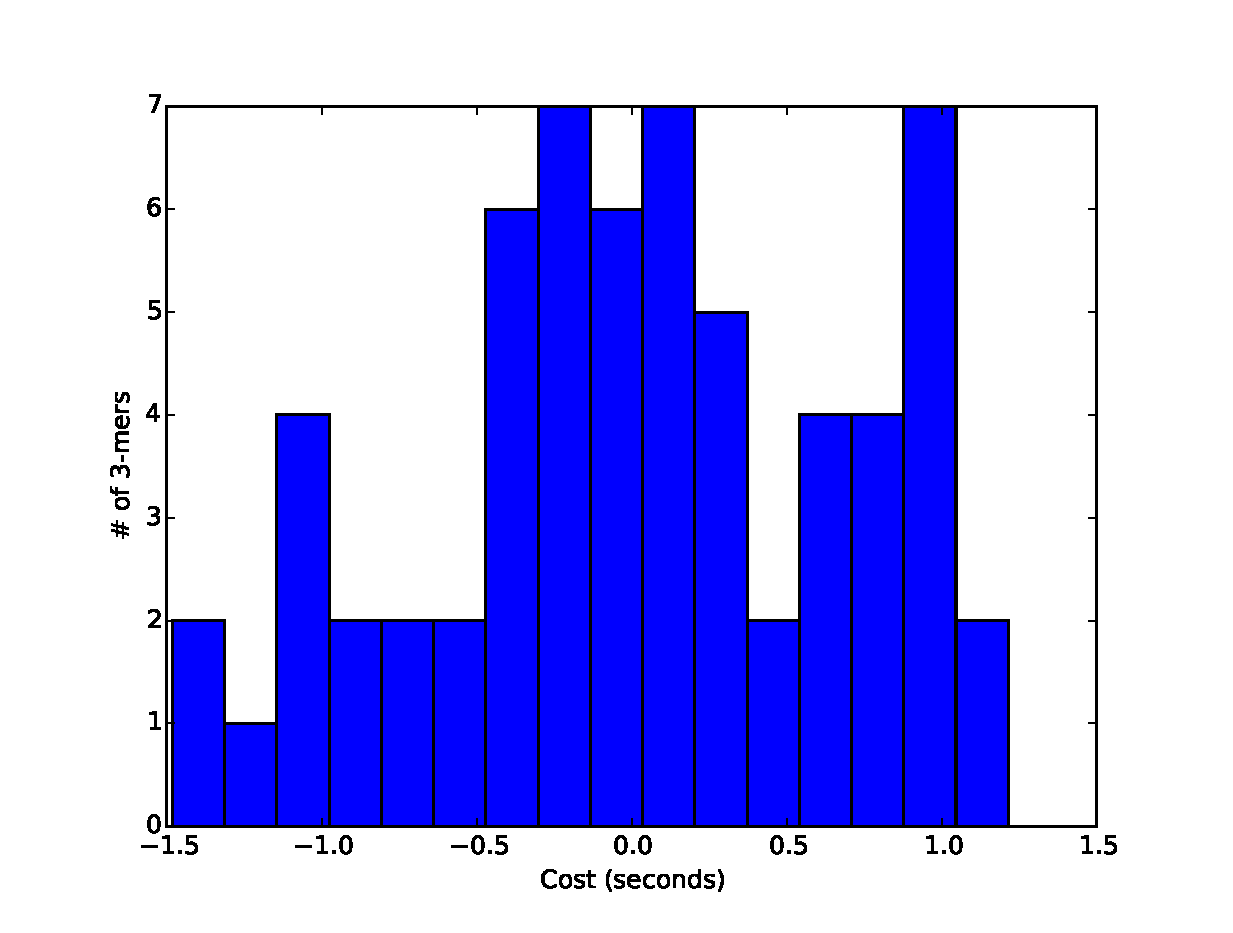
\includegraphics[width=3in]{part11hist3}
        \vspace{-70pt}
        \end{wrapfigure}
        We can use a model in which each the time to extend by one nucleotide is determined by the 3-mer in the middle of the
        pore.  We can not list all the costs, but here's a histogram:

        \vspace{1.5in}

        And here's the resulting predictions:
        
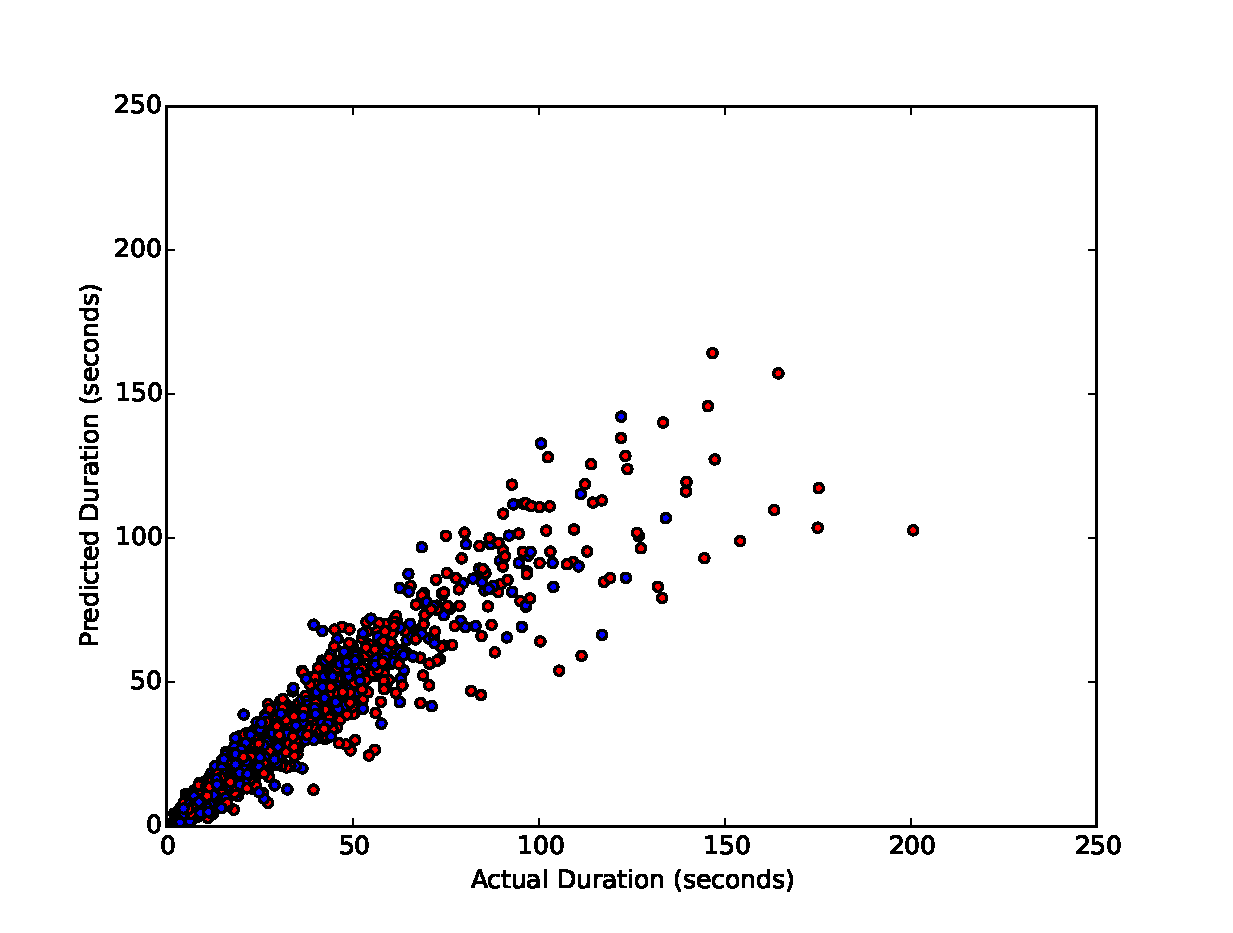
\includegraphics[width=\textwidth]{part11scatter3mer}

$r^2=0.91$


        \newpage
        \subsection*{4mer Model}
        \begin{wrapfigure}{R}{2in}
        \vspace{-50pt}
        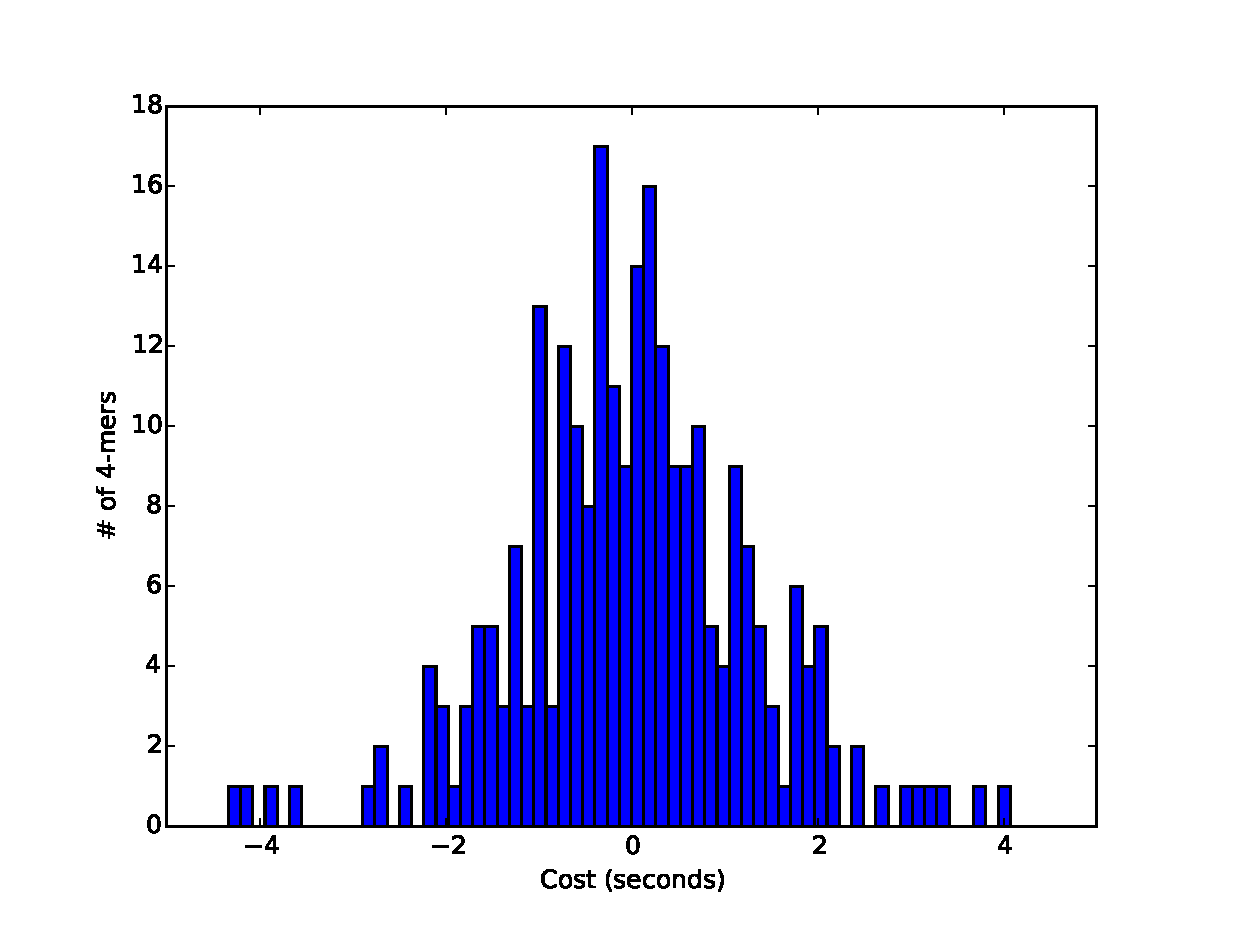
\includegraphics[width=3in]{part11hist4}
        \vspace{-70pt}
        \end{wrapfigure}
        We can use a model in which each the time to extend by one nucleotide is determined by the 4-mer in the middle of the
        pore.  We can not list all the costs, but here's a histogram:

        \vspace{1.5in}

        And here's the resulting predictions:
        
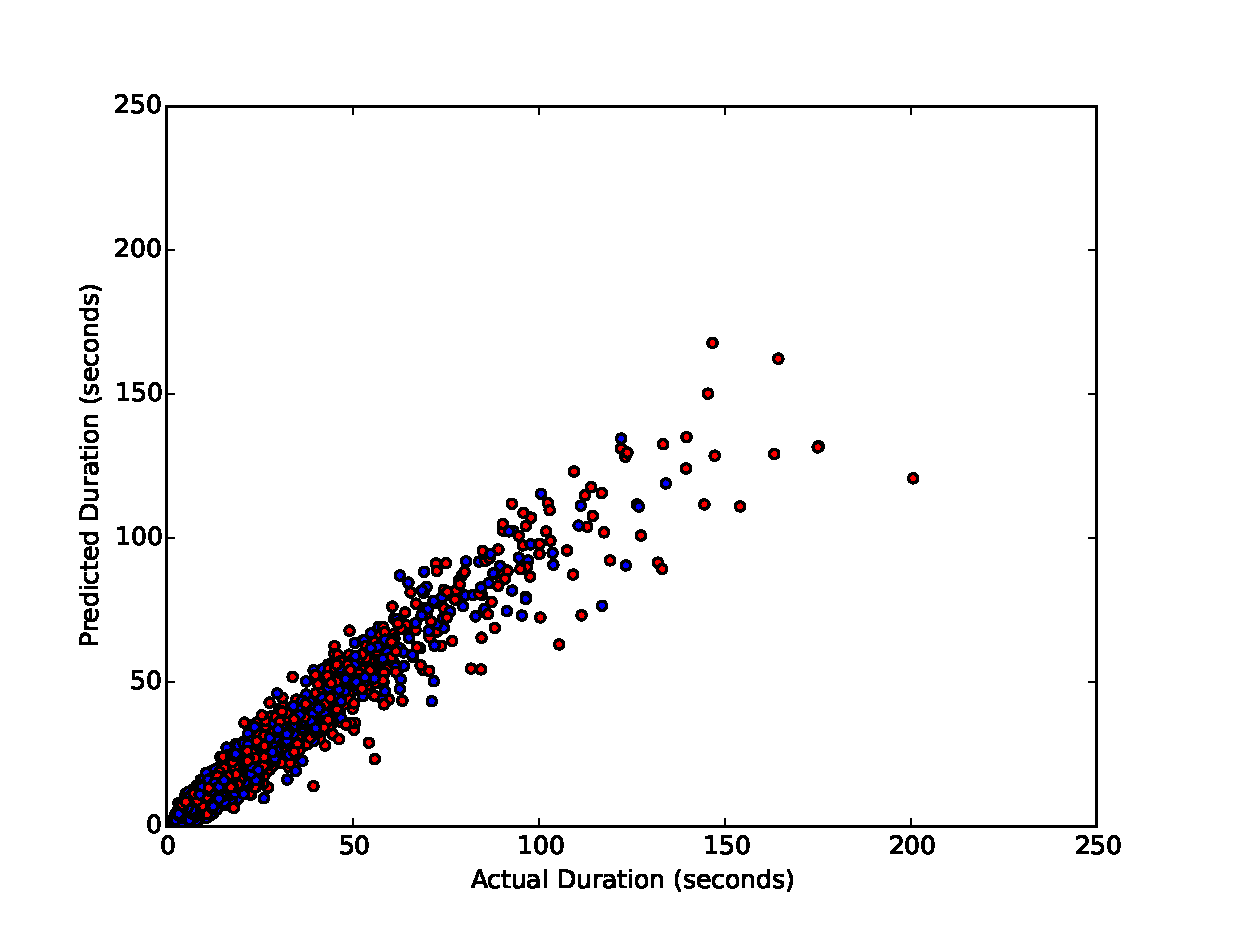
\includegraphics[width=\textwidth]{part11scatter4mer}

$r^2=0.94$


        \newpage
        \subsection*{5mer Model}
        \begin{wrapfigure}{R}{2in}
        \vspace{-50pt}
        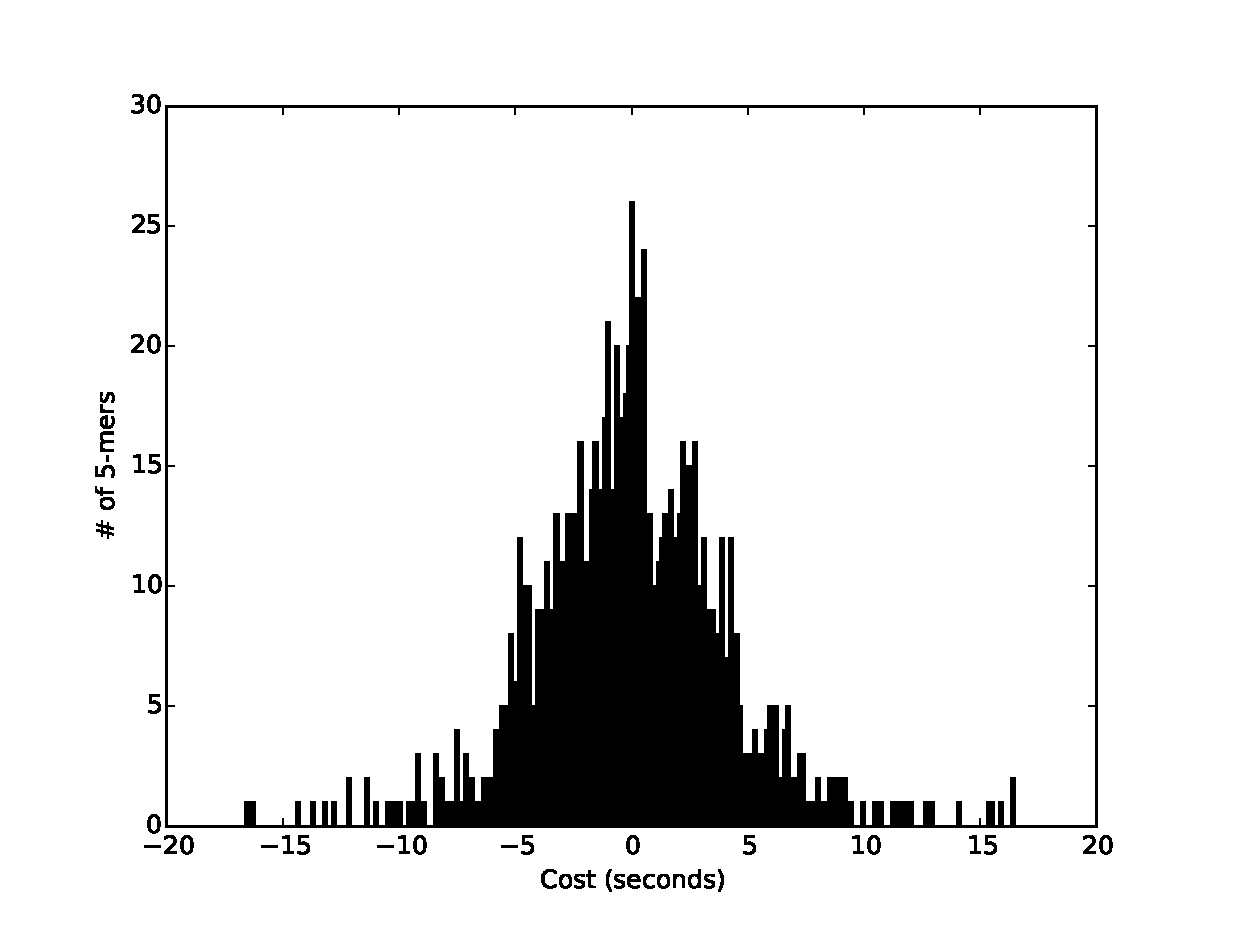
\includegraphics[width=3in]{part11hist5}
        \vspace{-70pt}
        \end{wrapfigure}
        We can use a model in which each the time to extend by one nucleotide is determined by the 5-mer in the middle of the
        pore.  We can not list all the costs, but here's a histogram:

        \vspace{1.5in}

        And here's the resulting predictions:
        
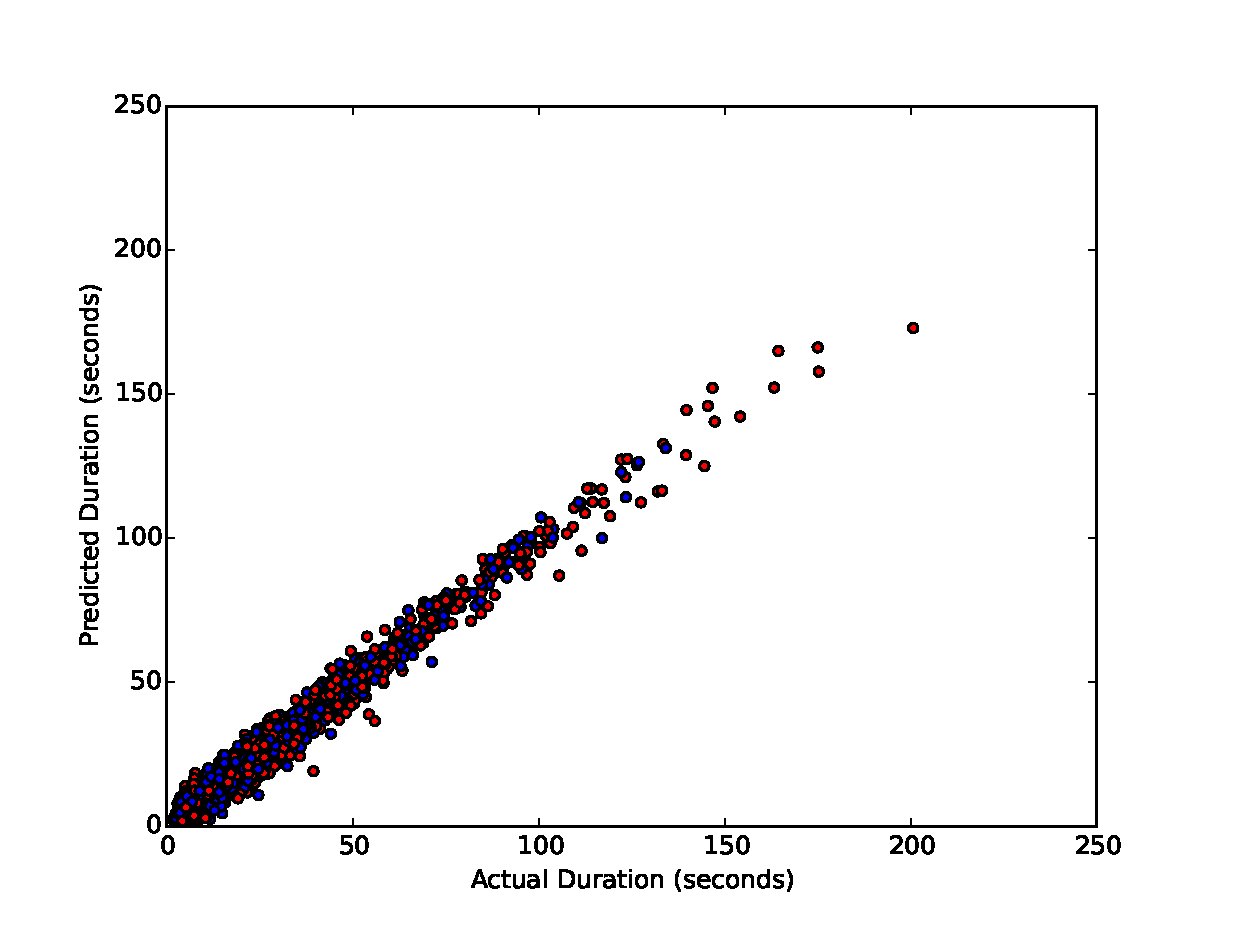
\includegraphics[width=\textwidth]{part11scatter5mer}

$r^2=0.98$



At this point our model has 1024 degrees of freedom for 2162 datapoints, so a good fit may reveal more overfitting than model appropriateness.
